\documentclass[letterpaper,11pt]{article}

% --- PAQUETES DE IDIOMA
\usepackage[spanish,mexico]{babel}
\usepackage[utf8]{inputenc}
\usepackage{csquotes}
\usepackage{iftex}

\usepackage{pdfpages}

% --- PAQUETES MATEMÁTICOS --
\usepackage{amsmath}
\usepackage{cancel}
\usepackage{mathrsfs}

% --- PAQUETES GRÁFICOS Y DE DISEÑO ---
\usepackage{graphicx}
\usepackage{float}
\usepackage{placeins}
\usepackage{subcaption}
\usepackage[table]{xcolor}
\usepackage{makecell}
\usepackage{array}
\usepackage{tikz}
\usetikzlibrary{shapes.geometric, shapes.multipart, positioning, arrows.meta, calc, shadows, decorations.pathreplacing,babel}

% --- LISTAS ---
\usepackage{enumitem}

% --- PAQUETES DE CÓDIGO ---
\usepackage{listings}
% Configuración del estilo de listings
\definecolor{codebg}{rgb}{0.95,0.95,0.95}   
\definecolor{keyword}{rgb}{0.0,0.2,0.6}     
\definecolor{comment}{rgb}{0.25,0.5,0.35}   
\definecolor{string}{rgb}{0.6,0.0,0.0}      
\definecolor{number}{rgb}{0.5,0.0,0.5}      
\definecolor{codegray}{rgb}{0.5,0.5,0.5}
\definecolor{codepurple}{rgb}{0.58,0,0.82}
\definecolor{backcolour}{rgb}{0.95,0.95,0.95}

\lstset{
  backgroundcolor=\color{backcolour},
  basicstyle=\ttfamily\small,
  keywordstyle=\color{blue}\bfseries,
  stringstyle=\color{codepurple},
  commentstyle=\color{codegray}\itshape,
  numbers=left,
  numberstyle=\tiny\color{codegray},
  frame=single,
  rulecolor=\color{black},
  breaklines=true,
  tabsize=4,
  showstringspaces=false,
  literate={á}{{\'a}}1
           {é}{{\'e}}1
           {í}{{\'i}}1
           {ó}{{\'o}}1
           {ú}{{\'u}}1
           {Á}{{\'A}}1
           {É}{{\'E}}1
           {Í}{{\'I}}1
           {Ó}{{\'O}}1
           {Ú}{{\'U}}1
           {ñ}{{\~n}}1
           {Ñ}{{\~N}}1
           {¿}{{\textquestiondown}}1
           {¡}{{\textexclamdown}}1
}

% Estilo para código en C
\lstdefinestyle{cstyle}{
  language=C,
  backgroundcolor=\color{backcolour},
  basicstyle=\ttfamily\small,
  keywordstyle=\color{blue}\bfseries,
    keywordstyle=[2]\color{yellow!70!orange}\bfseries,
    morekeywords=[2]{MPI_Init,MPI_Comm_size,MPI_Comm_rank,MPI_Send,MPI_Recv,MPI_Scatter,MPI_Gather,MPI_Bcast,MPI_Reduce,MPI_Finalize},
    emph={printf},
    emphstyle=\color{blue}\bfseries,
  stringstyle=\color{codepurple},
  commentstyle=\color{codegray}\itshape,
  numbers=left,
  numberstyle=\tiny\color{codegray},
  frame=single,
  rulecolor=\color{black},
  breaklines=true,
  tabsize=4,
  showstringspaces=false
}

% Definición del lenguaje Python para listings
\lstdefinelanguage[LAB]{Python}{
    morekeywords={False, None, True, and, as, assert, async, await, break,
                                class, continue, def, del, elif, else, except, finally,
                                for, from, global, if, import, in, is, lambda, nonlocal,
                                not, or, pass, raise, return, try, while, with, yield,
                                machine, Pin, PWM, ADC, Timer, sleep_ms, sleep_us},
    morecomment=[l]{\#},
    morestring=[b]",
    morestring=[b]',
    sensitive=true
}

% Estilo para salidas de consola/terminal
\lstdefinestyle{output}{
  backgroundcolor=\color{black!5},
  basicstyle=\ttfamily\footnotesize,
  numbers=none,
  frame=single,
  rulecolor=\color{black!30},
  breaklines=true,
  tabsize=4,
  showstringspaces=false,
  xleftmargin=0.5cm,
  xrightmargin=0.5cm
}

% --- ESTILOS PARA DIAGRAMAS DE FLUJO (TIKZ) ---
\tikzset{
  startstop/.style={rectangle, rounded corners, minimum width=3cm, minimum height=1cm,text centered, draw=black, fill=red!30},
  process/.style={rectangle, minimum width=3cm, minimum height=1cm, text centered, draw=black, fill=orange!30},
  decision/.style={diamond, aspect=2, minimum width=3cm, minimum height=1cm, text centered, draw=black, fill=green!30},
  io/.style={trapezium, trapezium left angle=70, trapezium right angle=110, minimum width=3cm, minimum height=1cm, text centered, draw=black, fill=blue!30},
  arrow/.style={thick,->,>=stealth}
}


\definecolor{azulresultado}{HTML}{0072C6}
\definecolor{rojoacarreo}{HTML}{FF0000}

% --- RUTAS DE IMÁGENES ---
\graphicspath{{img/}{portada_img/}}

\definecolor{armblue}{RGB}{0, 113, 188}

% --- ÍNDICE CON PUNTOS ---
\usepackage{tocloft}
\renewcommand{\cftsecleader}{\cftdotfill{\cftdotsep}}

% --- CONFIGURACIÓN DE PÁGINA (GEOMETRÍA) ---
\usepackage[
    left=25mm, 
    right=25mm,
    top=35mm,
    bottom=30mm,
    headheight=77pt, 
    papersize={21.59cm,27.94cm}
]{geometry}

% --- FORMATO DE TEXTO ---
\usepackage{setspace}
\onehalfspacing
\usepackage{parskip} 
\usepackage{lipsum}  

% --- VARIABLES GLOBALES ---
\newcommand{\materia}{}

% --- ENCABEZADOS Y PIES DE PÁGINA ---
\usepackage{fancyhdr}
\pagestyle{fancy}
\fancyhf{} 
\fancyhead[L]{
\includegraphics[height=1.5cm]{portada_img/der.png}}
\fancyhead[R]{
\includegraphics[height=1.5cm]{portada_img/izq.png}}
\fancyfoot[C]{\thepage} 
\renewcommand{\headrulewidth}{0.4pt} 
\renewcommand{\footrulewidth}{0pt}  

% --- BIBLIOGRAFÍA ---
\usepackage[backend=biber, style=apa, sortcites, url=true]{biblatex}
\addbibresource{referencias.bib}

% --- HIPERVÍNCULOS ---
\usepackage{hyperref}
\hypersetup{
    colorlinks=true,
    linkcolor=blue,
    citecolor=blue,
    filecolor=magenta,
    urlcolor=cyan
}

\begin{document}

\input{portada.tex}

\newpage
{\hypersetup{linkcolor=black}\tableofcontents}


\newpage

\setcounter{page}{1}
\singlespacing

\section{Parte 1. Análisis Estadístico con Excel}

\subsection{Creacion del excel a partir del documento dado:}

\begin{figure}[H]
    \centering
    
\includegraphics[width=0.8\textwidth]{image/part1/image1.png}
    \caption{Seleccion del archivo csv.}
    \label{fig:tabla_excel}
\end{figure}

\begin{figure}[H]
    \centering
    
\includegraphics[width=0.8\textwidth]{image/part1/image2.png}
    \caption{Seleccion del aasistente en delimitados.}
    \label{fig:tabla_excel2}
\end{figure}

\begin{figure}[H]
    \centering
    
\includegraphics[width=0.8\textwidth]{image/part1/image3.png}
    \caption{Seleccion de delimitador de coma.}
    \label{fig:tabla_excel3}
\end{figure}

\begin{figure}[H]
    \centering
    
\includegraphics[width=0.8\textwidth]{image/part1/image4.png}
    \caption{Seleccion de formato de columnas en general.}
    \label{fig:tabla_excel4}
\end{figure}

\begin{figure}[H]
    \centering
    
\includegraphics[width=0.8\textwidth]{image/part1/image5.png}
    \caption{Tabla generada en Excel.}
    \label{fig:tabla_excel5}
\end{figure}

\subsection{Creacion de tablas pivotes o tablas dinamicas recomendadas}

En este caso al ser el trabajo desde una MAC, en este caso la tabla generada alteroariamente fue esta:

\begin{figure}[H]
    \centering
    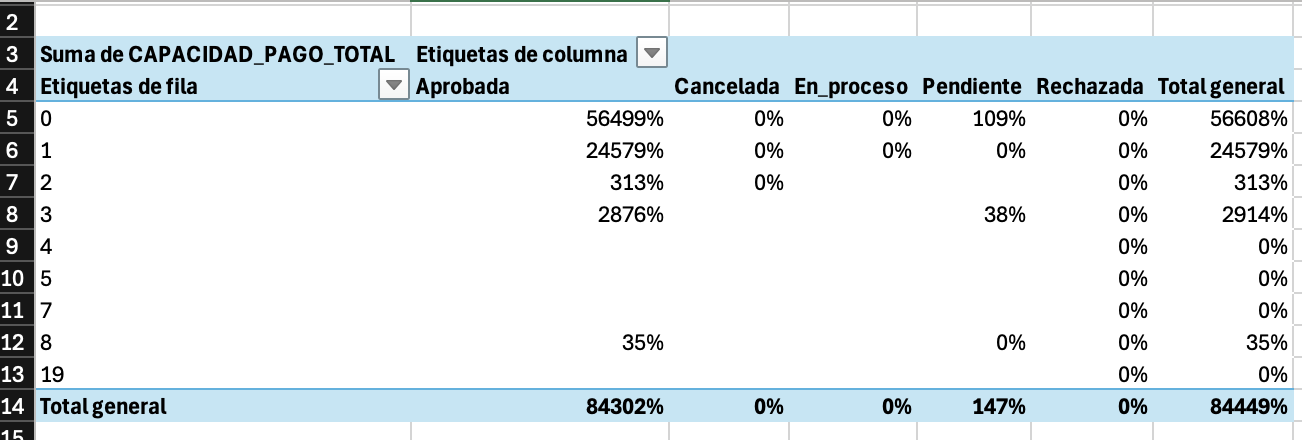
\includegraphics[width=0.8\textwidth]{image/image1.png}
    \caption{Tabla Pivote generada en Excel.}
    \label{fig:tabla_pivote}
\end{figure}

La tabla dinamica que se selecciono, en este caso, tenemos las columnas 
de etiquetas de la fila, que tienen a aprobadas, cancelada, en proceso, pendiente, rechazada y total general, para esto
casi todo se concentrada en las etiquetas que fueron aprobadas, en este caso con un 84,302\% del 84,449\% general, no obstante tenemos las solicitudes que estan marcadas 
como canceladas, en proceso y rechazada, que refleja un valor del 0\% a lo largo de todas las filas que estas tienen.

Este comportamiento nos dice directametne que en la captura de los datos, solo se conservan para los perfiles 
o personas que logran pasar por todos los filtros sin ningun problema para que se conserve en la base de datos, es por esto; que  provocaria que dejara en 0 las cuentas 
rechazadas, ademas de esto la distribucion nos dice que el grupo 0 y 1, son los que aportan la mayor parte de este valor, dimuyendo de forma agresiva a partir de la categoria 2.

\subsection{Creacion de tablas pivote o tablas dinamicas}

\textbf{Cuales son los valores que maneja la columna ESCOLARIDAD?}

\begin{figure}[H]
    \centering
    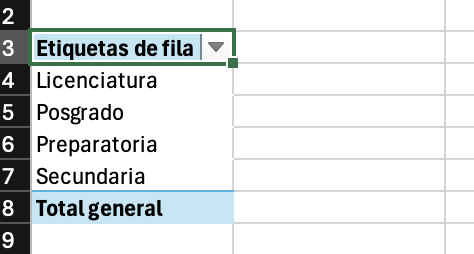
\includegraphics[width=0.8\textwidth]{image/image2.png}
    \caption{Tabla Pivote generada en Excel.}
    \label{fig:tabla_pivote2}
\end{figure}

La tabla columna escolaridad maneja los valores de los diferentes niveles, en este caso son 
los de Secundaria, Preparatoria y Licenciatura.

\textbf{Generacion de primera tabla}

\begin{figure}[H]
    \centering
    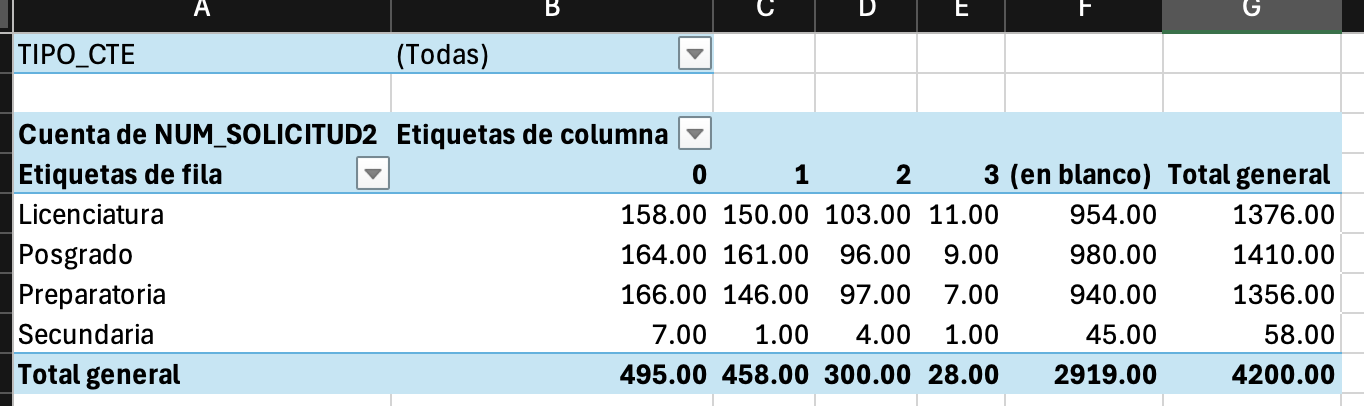
\includegraphics[width=0.8\textwidth]{image/image3.png}
    \caption{Tabla Pivote generada en Excel.}
    \label{fig:tabla_pivote3}
\end{figure}

\subsection{Interpretacion de la tablas pivote o tablas dinamicas}

\textbf{Interpretacion de la tabla \ref{fig:tabla_pivote3}}

En este caso la tabla nos dice que esta generada a partir de un recuento de 4200 registros, que son las solicitudes de credito,
distribuidas directamente segun el nivel de escolaridad que tiene cada persona o cliente directamente, en este caso al analizar todos los datos 
se ve destacado directamente desctacado, que casi todos los registros donde estamos hablando de unos 2919 de estos, se centran directametne en la categoria de meses vencidos ``En blanco'',
lo que nos dice que la mayoria de clientes recientes sin historial generado. Ahora bien, respecto a la distribucion demografica, 
el mayor numero de solicitudes
proviene de perfiles con nivel académico de 
"Posgrado" (1,410), seguido por 
"Licenciatura" (1,376) y
"Preparatoria" (1,356), 
mientras que la participación del nivel "Secundaria" 
es marginal con apenas 58 registros. 
Ya por ultimo tenemos el caso del
comportamiento de pago de los clientes que 
sí cuentan con un historial, 
la tendencia de estos es positiva, esto es por que
la mayor concentración se 
encuentra al corriente con cero meses vencidos 
que son alrededor de 495 clientes 
o presenta un atraso inicial de un mes que son alredeor de 
458 clientes. 

Esta incidencia va bajando directamente
conforme aumenta el tiempo de impago, 
llegando a solo 28 clientes que presentan 
el nivel más crítico de morosidad con tres meses vencidos.

\textbf{Generacion de grafica a partir de la tabla pivote}

\begin{figure}[H]
    \centering
    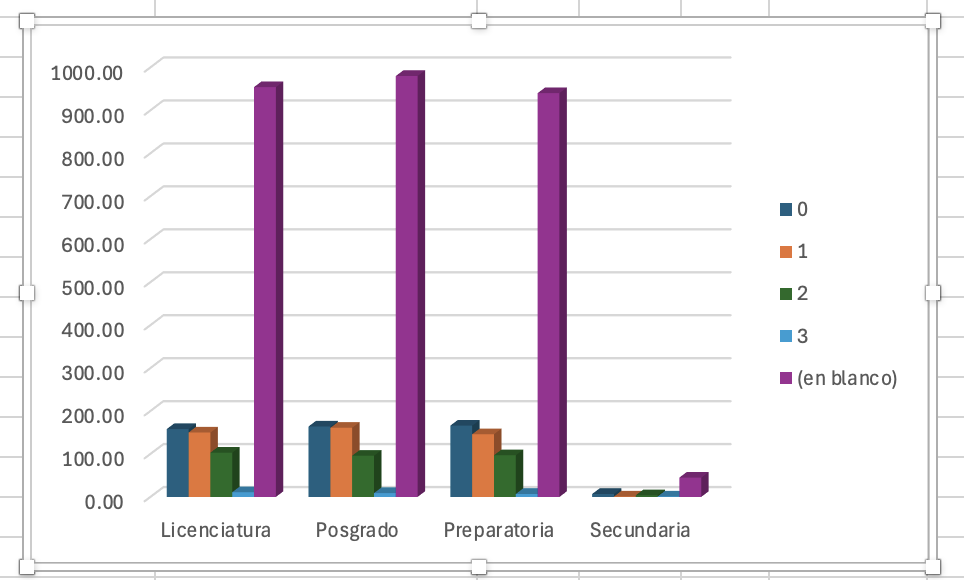
\includegraphics[width=0.8\textwidth]{image/image4.png}
    \caption{Grafica generada a partir de la tabla pivote en Excel.}
    \label{fig:grafica_pivote}
\end{figure}

\newpage
\textbf{Interpretacion de la grafica \ref{fig:grafica_pivote}}

En este caso la grafica nos dice de forma visual los resultados obtenidos en la tabla pivote, para esto casi todo se concentra en la barra de color morado que representa la categoria ``(en blanco)'', lo que nos dice directamente que la mayor parte de las solicitudes de todos los niveles educativos, salvo en secundaria, recaen en los clientes recientes sin historial. Ademas de esto la distribucion nos dice que el grupo 0 y 1, son los que aportan la mayor parte del resto de solicitudes, disminuyendo de forma agresiva a partir de la categoria 2 y 3, que presentan el nivel mas critico de morosidad.

Las columnas más pequeñas, se aprecia un claro efecto de "escalera descendente" de izquierda a derecha. La columna azul oscuro (0 meses) es la más alta de este subgrupo, seguida muy de cerca por la naranja (1 mes). A partir de ahí, la caída es drástica hacia la columna verde (2 meses) y la azul claro (3 meses) es apenas perceptible. Esto demuestra gráficamente que conforme aumenta la gravedad del atraso, el número de clientes que incurren en él es significativamente menor.



\subsection{Análisis de información utilizando tablas pivóte o tablas dinámicas}

A continuación se da respuesta a las preguntas solicitadas con base en el análisis de los datos correspondientes al tipo de cliente, estatus de la solicitud y meses vencidos:

\begin{itemize}
    \item \textbf{¿Cuántos clientes buenos tienen una cuenta aprobada con 3 meses vencidos?} \underline{\hspace{0.5cm}\textbf{0 clientes}\hspace{0.5cm}}
    
    En este caso, al revisar el cruce de los datos para los clientes clasificados como \textbf{BUENO} que tienen una cuenta \textbf{Aprobada}, se tiene que ninguno de ellos presenta 3 meses vencidos (0 clientes). Esto nos dice directamente que los clientes con buen perfil crediticio mantienen un comportamiento controlado y no llegan al nivel más crítico de morosidad, concentrando sus atrasos únicamente en 0, 1 y 2 meses.
    
    \item \textbf{¿Cuánto clientes regulares tienen una cuenta aprobada con 0 meses vencidos?} \underline{\hspace{0.5cm}\textbf{236 clientes}\hspace{0.5cm}}
    
    Para este caso, al analizar la información de los clientes catalogados como \textbf{REGULAR} que cuentan con su solicitud en estatus de \textbf{Aprobada}, se identifica que un total de \textbf{236 clientes} se encuentran completamente al corriente con 0 meses vencidos. Esto nos demuestra que una parte muy importante de los clientes regulares mantiene sus pagos al día y sin atrasos generados.
\end{itemize}

\textbf{Generacion de tabla dinamica}

\begin{figure}[H]
    \centering
    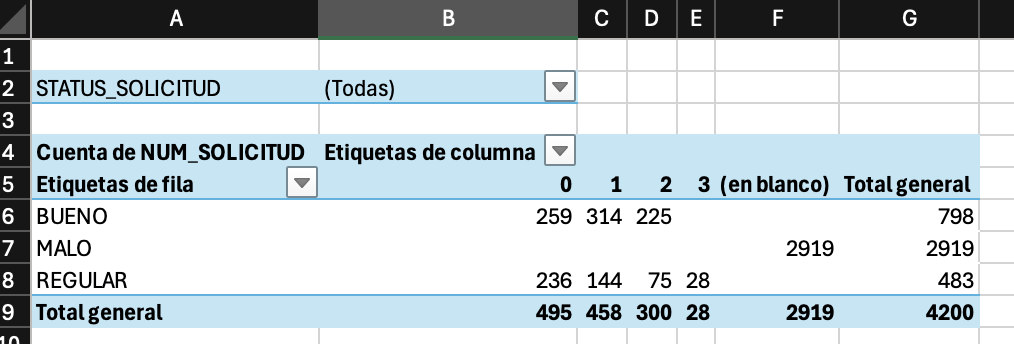
\includegraphics[width=0.7\textwidth]{image/image5.png}
    \caption{Tabla Dinamica generada en Excel.}
    \label{fig:tabla_pivote5}
\end{figure}

\textbf{Interpretacion de la tabla \ref{fig:tabla_pivote5}}

En este caso la tabla nos dice que está generada a partir 
de un total de 4200 registros, esto mediante una calsificacion que es
bueno, malo, regular y sus meses vencidos. 
En este caso al analizar todos los datos se ve 
destacado directamente que la gran mayoría de los registros, 
los cuales son de 2919 de estos, 
se centran directamente en la etiqueta ``(en blanco)'' 
que son relacionados directamente para los clientes 
con el perfil ``MALO''. 


Ahora bien, el comportamiento de pago de los clientes 
que sí cuentan con historial, 
la tendencia de estos nos muestra variaciones importantes. 
Para el perfil ``BUENO'', los pagos se concentran 
directamente en 1 mes que son de 314 registros y 0 
meses vencidos con 259 registros, 
llegando hasta los 2 meses sin tocar para nada el 
nivel crítico de 3 meses. 
Ya por último tenemos el caso de los clientes con perfil ``REGULAR'', 
donde la tendencia es muy positiva desde el inicio, esto es porque la mayor concentración se encuentra al corriente con cero meses vencidos que son alrededor de 236 clientes. 

\textbf{Generacion de grafica a partir de la tabla dinamica}

\begin{figure}[H]
    \centering
    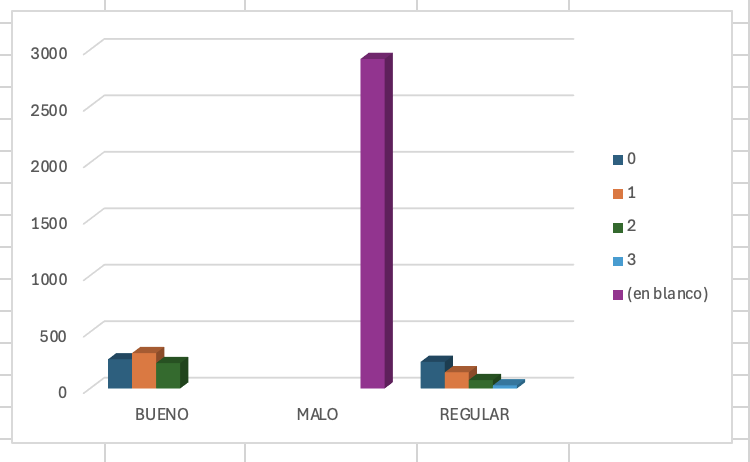
\includegraphics[width=0.6\textwidth]{image/image6.png}
    \caption{Grafica generada a partir de la tabla dinamica en Excel.}
    \label{fig:grafica_pivote6}
\end{figure}

\textbf{Interpretacion de la grafica \ref{fig:grafica_pivote6}}

En este caso la grafica nos dice, que nuestra intretacion de los datos es correcta,
esto por que casi todo el volumen se concentra 
de forma casi total en la barra morada que representa la parte de en blanco
dentro del perfil ``MALO''. 

Ya por ultimo, las columnas más pequeñas de los demas casos, 
para la categoría de clientes regulares 
se aprecia como van descendiendo como si fuera una escalera 
esto de izquierda a derecha. 
En cambio, para los clientes buenos, 
la barra naranja de 1 mes supera a la azul,
lo que nos dice que tiene condiciones que evitan que 
incurran en el nivel más crítico de morosidad.

\subsection{Conclusion (Parte 1)}

En este caso, a lo largo de toda esta parte 1 de la practica, 
el uso y creación de tablas dinámicas me ayudo a comprender
cómo transformar muchos datos exparcidos en información 
que puedo interpretar por medio de las tablas y graficos. 
Al analizar los 4200 registros, 
pude identificar comportamientos, como en los cuales 
note que la gran mayoría de los datos se 
concentran en cuentas sin historial bajo la etiqueta 
que son las en blanco en este caso.

\section{Parte 2. Análisis Estadístico con PowerBI}


\newpage

% Impresión Referencias
\nocite{*}
\printbibliography[heading=bibintoc, title={Referencias}]

\end{document}